%Thus far in this work a solution to simplify and automate design the process of all digital PLL loop filter designs comprised of (1) an automated loop filter optimization and design engine, and (2) a discrete-event, time domain PLL simulator to evaluate the designed filters with full time-discretization and quantization nonlinearity effects. I
In this discussion, the performance of the implemented design will first be analyzed via comparison to current state of art. Small area and low power PLLs are considered for reference.

\subsection{State of art}


SSCL'20 Liu cheats because it is not quadrature, power is 108 muW for one phase...

JSSC'19 Liu Requires long calibration for TDC (1024 samples), slow??

Need 2x stage at 2.4 GHz for IQ, make new metric for this....


	\begin{table}[h!]
		\centering
		\def\arraystretch{1.5}		
		\setlength\arrayrulewidth{0.75pt}
		\setlength{\tabcolsep}{0.5em} % for the horizontal padding
		\begin{tabular}{|>{\centering}m{0.2\textwidth}?>{\centering}m{0.1\textwidth}?>{\centering}m{0.11\textwidth}|>{\centering}m{0.1\textwidth}|>{\centering}m{0.1\textwidth}?>{\centering}m{0.11\textwidth}|>{\centering\arraybackslash}m{0.1\textwidth}|}
			\hline 
			\rule[-1ex]{0pt}{2.5ex} \cellcolor{gray!40}\textbf{Parameter} & \cellcolor{gray!40}\textbf{This Work} & \cellcolor{gray!40}\textbf{JSSC'19 Liu} \cite{Liu2019} & \cellcolor{gray!40}\textbf{{\footnotesize NORCHIP'18 Palaniappan} }\cite{Palaniappan2018} & \cellcolor{gray!40}\textbf{SSCL'20 Liu} \cite{Liu2020} & \cellcolor{gray!40}\textbf{2019 Zhang} \cite{Zhang2019} & \cellcolor{gray!40}\textbf{CICC'20 Xiang} \cite{Xiang2020} \\
			\hline 
			\rule[-1ex]{0pt}{2.5ex} \textbf{Analog/Digital} & Digital  & Digital  & Digital & Digital & Analog & Analog \\
			\hline 
			\rule[-1ex]{0pt}{2.5ex} \textbf{Int-N/Frac-N} & Int-N  & Frac-N  & Int-N & Int-N & Int-N & Int-N  \\
			\hline 
			\rule[-1ex]{0pt}{2.5ex} \textbf{Architecture} & BB-PLL\tablefootnote{BBPD PLL} & FLL + ODZ\tablefootnote{Out of deadzone}  & {Digital CP-PLL\tablefootnote{Charge Pump PLL}} & IL-PLL\tablefootnote{Injection-locked PLL} & CP-PLL & CP-PLL \\
			\hline 
			\rule[-1ex]{0pt}{2.5ex} \textbf{Process} & 22nm & 65nm & 40nm & 5nm & 40nm & 22nm \\
			\hline 
			\rule[-1ex]{0pt}{2.5ex} \textbf{Osc. Type} & RO & LC & RO & RO & RO  & RO \\
			\hline 
			\rule[-1ex]{0pt}{2.5ex} \textbf{Detector} & BBPD & ODZ & PFD\tablefootnote{Phase-frequency detector} & Sampling & PFD & PFD\\
			\hline
			\rule[-1ex]{0pt}{2.5ex} \textbf{Area [mm$^2$]} & 0.0051 & 0.25 & 0.0186 & 0.0036 & 0.00873 & 0.015 \\
			\hline 
			\rule[-1ex]{0pt}{2.5ex} \textbf{Power [$\mu$W]} & 100 & 265 & 270.5 & 440 & 170  & 682 \\
			\hline 		 
			\rule[-1ex]{0pt}{2.5ex} \textbf{f$_{ref}$ [MHz]} & 16 & 10 & - & 40 & 100 & 20-200 \\
			\hline 
			\rule[-1ex]{0pt}{2.5ex} \textbf{f$_{osc}$ [GHz]} & 0.816 & 2.1-3.1 & 330-470 & 1.0 & 1.6 & 3.2 \\
			\hline 
			\rule[-1ex]{0pt}{2.5ex} \textbf{Osc. Stages (N$_{stg}$)} & 6 & 1 & 8 & - & 3 & - \\
			\hline 
			\rule[-1ex]{0pt}{2.5ex} \textbf{f$_{osc}$ $\times$ N$_{stg}$} [GHz] & 4.896 & 2.1-3.1 & 2640-3760 & - & 0.45-4.8 & - \\
			\hline 	
			\rule[-1ex]{0pt}{2.5ex} \textbf{Osc. Power [$\mu$W]} & 80 & 107 & - & 398 & - & 225 \\
			\hline 		
			\rule[-1ex]{0pt}{2.5ex} \textbf{Jitter [ps$_{RMS}$]} & 15.1  & 2.8 & 9.53 & 2.34 & 8.3 & 2.3 \\
			\hline 			
			\rule[-1ex]{0pt}{2.5ex} \textbf{$\textnormal{FOM}_{\textnormal{jitter}}$ [dB]} & -226.5  &  -236.8 & -226.1 & -236.2 & -229.3 & -234.3 \\
			\hline 		
			\rule[-1ex]{0pt}{2.5ex} \textbf{Lock-time [$\mu$s]} & $\leq$ \hl{X} & $\leq$ 120  & - & - & - & 0.2 \\
			\hline 			
		\end{tabular} 
		% \caption{Assigned specifications for branch line hybrid design.}
		% \label{asgn_specs}
		\caption{PLL parameters determined from filter design and optimization process for minimum phase noise with BBPD.}
		\label{tab:state_of_art}
	\end{table}  

	\begin{figure}[htb!]
	    \centering
	    \begin{subfigure}{0.5\textwidth}
	        \centering
	        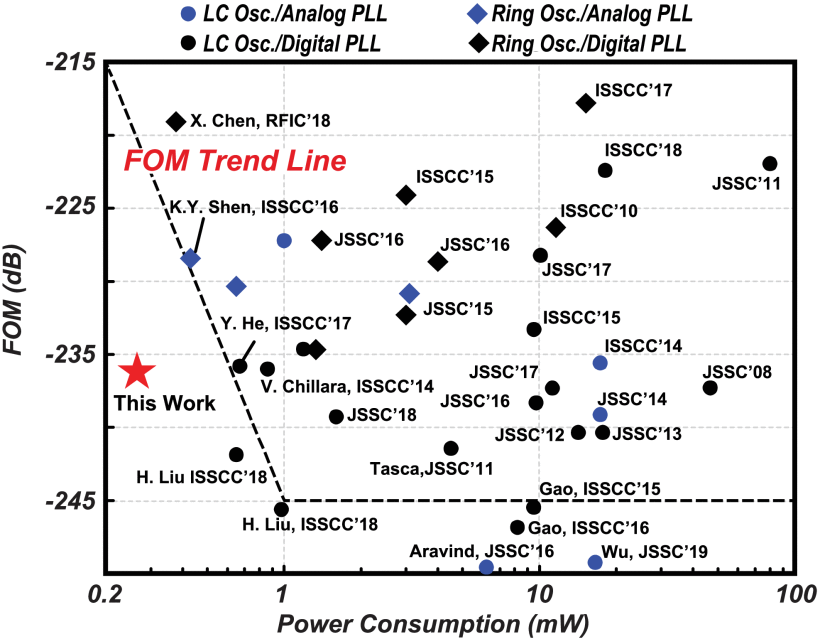
\includegraphics[width=1\textwidth, angle=0]{./figs/liu24-fom}
	        \caption{ }
	        \label{fig:fom_v_pow}
	    \end{subfigure}%
	    \begin{subfigure}{0.5\textwidth}
	        \centering
	        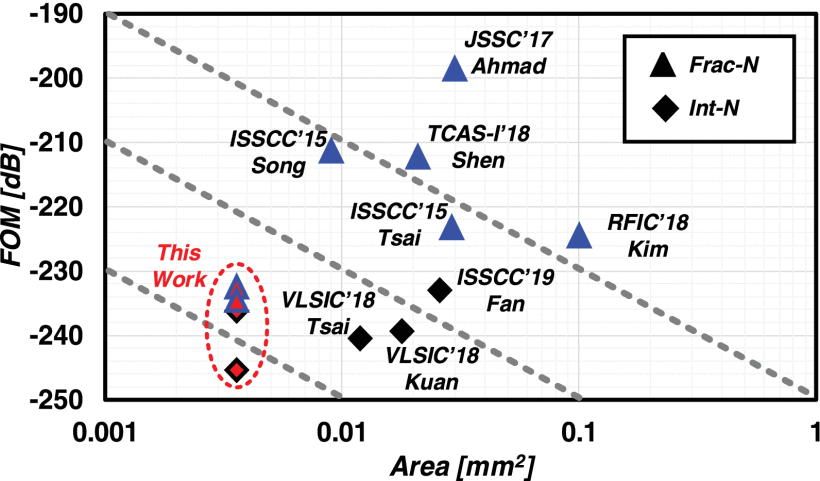
\includegraphics[width=1\textwidth, angle=0]{./figs/liu_5nm}
	        \caption{ }
	        \label{fig:fom_v_area}
	    \end{subfigure}
	    \caption{\textbf{(a)} FOM$_{jitter}$ versus power from \cite{Liu2019} (JSSC 2019), \textbf{(b)} FOM$_{jitter}$ versus area from \cite{Liu2020} (SSCL 2020).}
	    \label{fig:fom_charts}
	\end{figure}


	% \begin{figure}[htb!]
	% 	\center\includegraphics[width=1.0\textwidth, angle=0]{figs/x.pdf}
	% 	\caption{Transient simulation of optimal design.}
	% 	\label{fig:des_ex_trans}
	% \end{figure}
	% \FloatBarrier

	% \begin{figure}[htb!]
	% 	\center\includegraphics[width=1.0\textwidth, angle=0]{figs/x.pdf}
	% 	\caption{Variation Simulation for KDCO.}
	% 	\label{fig:var_lock}
	% \end{figure}
	% \FloatBarrier

	% \begin{figure}[htb!]
	% 	\center\includegraphics[width=1.0\textwidth, angle=0]{figs/x.pdf}
	% 	\caption{Phase noise.}
	% 	\label{fig:Simulated phase noise.}
	% \end{figure}
	% \FloatBarrier

	% stability criteria - Jurys' stability criteria abs(a0) l.t. a2 for second order z-transfer \cite{xiu_li_meiners_padakanti_2004}
	% - Not phase margin based in optimization, can make stable by using stable choice of PI controller (two poles only) - poles should be in unit circle...
\FloatBarrier

\subsection{Areas of improvement}
	\subsubsection{Coarse calibration}
	The coarse calibration scheme implemented is capacitor based, and does not provide robust enough tuning in the presence of process and voltage variation. The coarse implementation of this work allows for approximately 15\% fractional tuning range, where as standard deviation the simulated oscillator variance due to process variation under fixed biasing is 4.2 \% of the oscillator frequency. This results in coverage of $\pm$1.78$\sigma$ of the sample variance from the mean, or a yield of 92.5\% under ideal biasing. However, under non ideal biasing conditions, extra deviation of the oscillator frequency is inherent. It was observed from simulation that the oscillator frequency deviates by 2.588 MHz/mV of extra bias, or 0.3\% of the oscillator frequency per mV. A $V_{DD}$ offset of only 47.3 mV (6\% of 0.8V) to shift the oscillator by 15\%, enought that there is no expectation that the coarse calibration can correct the frequency range. 

	The current capacitor-based coarse calibration is limited due to the loading it exerts on the ring oscillator core. For a greater tuning range, a larger bank work would be required, however it was found during the design process that obtaining the correct frequency range under constrained power with acceptable phase noise was not possible with a larger capacitor bank. A highly viable solution to this problem is to use tuning of the supply voltage to implement coarse tuning, and to forgo the capacitor tuning bank all together. Removal of the capacitor bank will reduce oscillator core loading, thus increasing frequency of the oscillator. Longer channel lengths could be used in the oscillator core (again reducing frequency), to improve phase noise performance. Such a change would require implementation of a digitally tunable voltage regulator for the oscillator core, with tight regulation of supply voltage. Requirement of tight regulation of the supply is paramount due to the high frequency gain of the oscillator with supply tuning (again 2.588 MHz/mV, or 0.3\%/mV). Design of such a regulator within the PLL power requirements is possibly a daunting endeavor, and has been considered outside of the current scope of this work, as a possible future area of improvement.

	\subsubsection{Subharmonic oscillator}
		The usage of a 1/3 subharmonic oscillator as in this work is possibly undesirable in some regards for application to radio receiver design. This design choice pushes additional circuit complexity into receiver circuits, which must be designed to achieve full rate sampling by edge combining the 12 oscillator phases resulting from the 6-stage, 1/3 sub-harmonic oscillator. It is therefore probable that topological improvements for achieving full frequency operation of this PLL design for radio applications is a possible area of improvement. The removal of the capacitive tuning bank in the oscillator core, and utilization of supply tuning may allow for operating frequency for such an improvement to be realized.

	\subsubsection{CDAC switching noise}	
		It has been observed in the implemented CDACs that transient spikes occur in the DAC output during changing of the input code, as demonstrated in figure \ref{fig:dac_sw_noise}. This is a result of differing RC constants of the different switch and capacitor combinations.  The small RC constant switch and capacitor combinations will settle very fast, causing an inital rising/falling portion of a spike to be seen in the DCO ouput. The larger capacitor and switch combinations will settle delayed in time, causing the spike to subside and the output to settle to the desired value. The DCO spikes, while short in duration, are expected to have a contribution to increasing phase noise of the oscillator. An area of improvement in future is to reduce this spiking, though more careful design of the switch and capacitor combinations. 
		\begin{figure}[htb!]
	        \centering
	        \includegraphics[width=0.65\textwidth, angle=0]{example-image}
		    \caption{Noise tranients in DAC output during switching.}
		    \label{fig:dac_sw_noise}
		\end{figure}


\FloatBarrier
% \normalsize